\documentclass[11pt,a4paper]{article}
\usepackage[utf8]{inputenc}
\usepackage[margin=1in]{geometry}
\usepackage{amsmath}
\usepackage{hyperref}
\usepackage{listings}
\usepackage{xcolor}
\usepackage{tikz}
\usetikzlibrary{shapes,arrows,positioning,decorations.pathreplacing}

\title{Zed's Context Management Architecture: A Transparent Text-First Approach to LLM Context}
\author{Research Paper}
\date{November 17, 2025}

\begin{document}

\maketitle

\section{Introduction}

Unlike many AI-powered code editors that use hidden embedding systems and vector databases, Zed takes a radically transparent, text-first approach to context management. The language model sees exactly what the user sees in the Agent Panel or Text Threads—there are no opaque vector stores or secret RAG layers. This paper examines how Zed builds, manages, and delivers context to language models through its text-thread architecture, explicit context injection mechanisms, and observable automatic context gathering via tools.

\section{The Text-First Philosophy}

Zed's core principle is transparency: everything the LLM receives is visible in the Agent Panel or Text Threads. The context is built from explicit text blocks that users can see, edit, and control. There is no hidden embedding layer that automatically indexes the entire codebase.

\begin{itemize}
    \item \textbf{Text Threads}: The conversation is stored as editable text blocks (System, You, Assistant)
    \item \textbf{Explicit Context}: All context comes from manual inclusion or observable tool calls
    \item \textbf{No Hidden Memory}: The prompt is the thread—there is no invisible history
    \item \textbf{Editable History}: Users can rewrite any part of the conversation before resending
    \item \textbf{Automatic but Observable}: Agent-driven context gathering is visible, not hidden
\end{itemize}

This approach gives users complete control and visibility over what context the model receives, making it easier to debug, optimize, and understand model behavior.

\section{Thread-Based Context Architecture}

Zed's context management centers around two distinct thread types, each serving different purposes.

\subsection{Text Threads vs Agent Panel}

Zed provides two thread interfaces with different capabilities:

\begin{itemize}
    \item \textbf{Text Threads}: Editor-like, fully editable conversation documents. Support slash commands but have no tool calls or agentic behavior—they're "just chat" for simple Q\&A and file inspection workflows.
    \item \textbf{Agent Panel Threads}: Optimized for agentic workflows with @-mentions, tool calls, profiles, MCP integration, external agents, token meters, and summarization. This is where automatic context gathering and code editing happen.
\end{itemize}

Both use the same underlying text-thread architecture (editable System/You/Assistant blocks), but Agent Panel threads add the tool-calling layer that enables autonomous codebase traversal.

\begin{figure}[htbp]
\centering
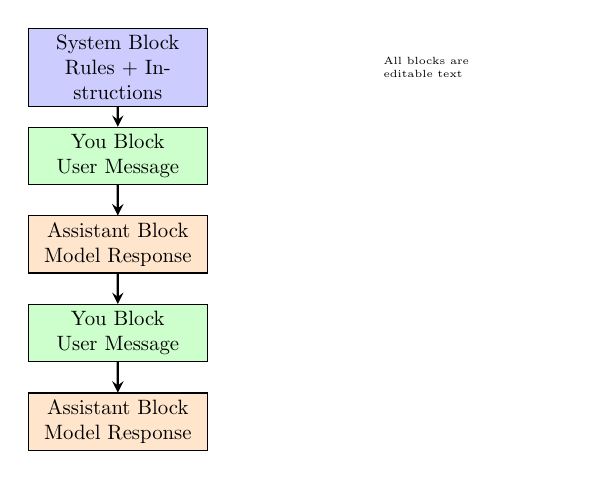
\begin{tikzpicture}[
    node distance=1.5cm,
    box/.style={rectangle, draw, text width=2.8cm, text centered, minimum height=0.8cm},
    system/.style={rectangle, draw, text width=2.8cm, text centered, minimum height=0.8cm, fill=blue!20},
    user/.style={rectangle, draw, text width=2.8cm, text centered, minimum height=0.8cm, fill=green!20},
    assistant/.style={rectangle, draw, text width=2.8cm, text centered, minimum height=0.8cm, fill=orange!20},
    arrow/.style={->, >=stealth, thick},
    scale=0.75,
    transform shape
]
    \node[system] (system) {System Block\\Rules + Instructions};
    \node[user, below of=system] (user1) {You Block\\User Message};
    \node[assistant, below of=user1] (assistant1) {Assistant Block\\Model Response};
    \node[user, below of=assistant1] (user2) {You Block\\User Message};
    \node[assistant, below of=user2] (assistant2) {Assistant Block\\Model Response};

    \draw[arrow] (system) -- (user1);
    \draw[arrow] (user1) -- (assistant1);
    \draw[arrow] (assistant1) -- (user2);
    \draw[arrow] (user2) -- (assistant2);
    
    \node[right of=system, xshift=4.5cm, text width=3cm, font=\tiny] {All blocks are\\editable text};
\end{tikzpicture}
\caption{Text Thread Structure}
\label{fig:thread}
\end{figure}

When a user sends a message, Zed converts these text blocks into a standard chat messages array (system, user, assistant) and sends it to the chosen provider. The thread itself is the prompt—there is no separate "memory" object.

\section{Building Context: Manual Injection Methods}

Zed provides explicit ways to inject context into threads. All methods result in literal text being inserted into the conversation.

\subsection{@-Mentions (Agent Panel Primary)}

In the Agent Panel, @-mentions are the primary mechanism for adding context:

\begin{itemize}
    \item @files – Mention specific files
    \item @directories – Mention entire directories
    \item @symbols – Mention code symbols
    \item @threads – Reference previous conversations
    \item @rules – Reference saved rule files
    \item Selection – Add current selection via @ menu
\end{itemize}

Mentions expand into tagged \texttt{<context>} blocks when building the request, clearly labeled so the LLM knows what was attached.

\subsection{Slash Commands (Text Threads \& Extensions)}

Slash commands are especially important in Text Threads and can be extended by extensions or external agents:

\begin{itemize}
    \item \texttt{/file <path>} – Inserts file contents or directory tree
    \item \texttt{/tab [name|all]} – Inserts current tab or all open tabs
    \item \texttt{/selection} – Inserts the current text selection
    \item \texttt{/diagnostics} – Inserts language-server diagnostics
    \item \texttt{/terminal [n]} – Inserts last N lines of terminal output
    \item \texttt{/now} – Inserts current date/time
    \item \texttt{/symbols} – Inserts symbol outline of current file
    \item \texttt{/prompt <name>} – Inserts saved rules
    \item \texttt{/fetch <url>} – Fetches content from HTTP endpoint
\end{itemize}

Extensions can provide custom slash commands (e.g., MCP servers, external agents like Claude Code). Slash commands are supported in rules files when used with Text Threads, but @-mentions are not supported inside rules files.

Important: Folds in the UI are just visual—the model still sees all the text. Token counts include folded content.

\begin{figure}[htbp]
\centering
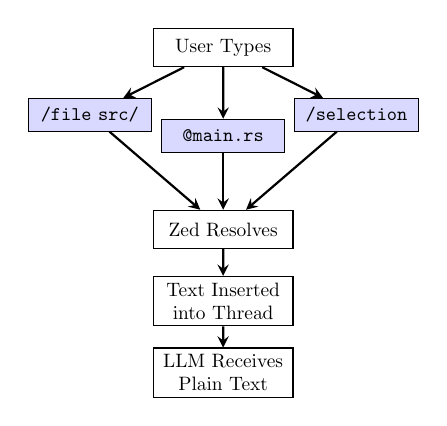
\begin{tikzpicture}[
    node distance=1.3cm,
    box/.style={rectangle, draw, text width=2.3cm, text centered, minimum height=0.7cm},
    command/.style={rectangle, draw, text width=2cm, text centered, minimum height=0.6cm, fill=blue!15},
    arrow/.style={->, >=stealth, thick},
    scale=0.7,
    transform shape
]
    \node[box] (user) {User Types};
    \node[command, below left of=user, xshift=-1.5cm, yshift=-0.3cm] (slash) {\texttt{/file src/}};
    \node[command, below of=user, yshift=-0.3cm] (mention) {\texttt{@main.rs}};
    \node[command, below right of=user, xshift=1.5cm, yshift=-0.3cm] (select) {\texttt{/selection}};
    \node[box, below of=user, yshift=-2cm] (resolve) {Zed Resolves};
    \node[box, below of=resolve] (insert) {Text Inserted\\into Thread};
    \node[box, below of=insert] (llm) {LLM Receives\\Plain Text};

    \draw[arrow] (user) -- (slash);
    \draw[arrow] (user) -- (mention);
    \draw[arrow] (user) -- (select);
    \draw[arrow] (slash) -- (resolve);
    \draw[arrow] (mention) -- (resolve);
    \draw[arrow] (select) -- (resolve);
    \draw[arrow] (resolve) -- (insert);
    \draw[arrow] (insert) -- (llm);
\end{tikzpicture}
\caption{Context Injection Flow}
\label{fig:injection}
\end{figure}

\section{System Prompt Construction}

The system prompt is built from multiple sources and is always prepended to every request.

\subsection{Rules and Project Context}

Zed automatically scans project directories for rule files matching patterns like:
\begin{itemize}
    \item \texttt{.rules}
    \item \texttt{.cursorrules}
    \item \texttt{.windsurfrules}
    \item \texttt{.clinerules}
    \item \texttt{.github/copilot-instructions.md}
    \item \texttt{AGENT*.md}, \texttt{CLAUDE.md}, \texttt{GEMINI.md}
\end{itemize}

\subsubsection{Rule Precedence and Limitations}

Zed uses only the first matching project rules file in a priority list (first match wins). Rules are project-level only—there's no built-in per-directory or per-file granularity. Rules Library entries don't apply automatically; you must explicitly @-mention them (\texttt{@rules}) in the Agent Panel.

Additionally, the system prompt includes:
\begin{itemize}
    \item Fixed instructions (communication style, tool usage rules)
    \item List of visible worktree roots
    \item Operating system, architecture, and shell information
    \item Model name and capabilities
\end{itemize}

\begin{figure}[htbp]
\centering
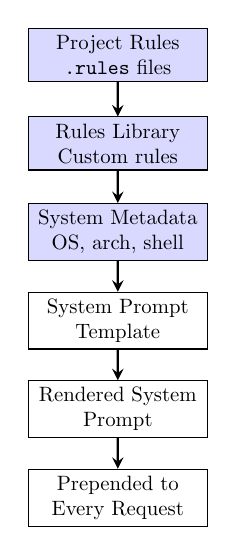
\begin{tikzpicture}[
    node distance=1.5cm,
    box/.style={rectangle, draw, text width=2.8cm, text centered, minimum height=0.8cm},
    source/.style={rectangle, draw, text width=2.8cm, text centered, minimum height=0.7cm, fill=blue!15},
    arrow/.style={->, >=stealth, thick},
    scale=0.75,
    transform shape
]
    \node[source] (rules) {Project Rules\\\texttt{.rules} files};
    \node[source, below of=rules] (library) {Rules Library\\Custom rules};
    \node[source, below of=library] (metadata) {System Metadata\\OS, arch, shell};
    \node[box, below of=metadata] (template) {System Prompt\\Template};
    \node[box, below of=template] (render) {Rendered System\\Prompt};
    \node[box, below of=render] (prepend) {Prepended to\\Every Request};

    \draw[arrow] (rules) -- (library);
    \draw[arrow] (library) -- (metadata);
    \draw[arrow] (metadata) -- (template);
    \draw[arrow] (template) -- (render);
    \draw[arrow] (render) -- (prepend);
\end{tikzpicture}
\caption{System Prompt Construction}
\label{fig:system}
\end{figure}

\section{Automatic Context via Tools}

While manual context injection gives users control, Zed's built-in agent can automatically gather context through tool calls. This is automatic but observable: the agent chooses which tools to call and which files to read, but all tool calls and their outputs appear as visible messages in the thread.

\subsection{Built-in Tools}

Zed's agent has access to tools that allow it to:
\begin{itemize}
    \item Read files from the project
    \item Search the codebase for symbols
    \item Run terminal commands
    \item Edit files (as discussed in the smart edit paper)
    \item List directories
\end{itemize}

When the agent calls a tool, the tool's output is added as a context message in the conversation. The agent can see these results and use them to generate its response. This automatic traversal is transparent—unlike hidden embedding systems, you see every file read and every tool call.

\subsection{Profiles}

Zed provides different profiles (Write, Ask, Minimal) that control which tools are available:
\begin{itemize}
    \item \textbf{Write}: Full tool access including file editing
    \item \textbf{Ask}: Read-only tools (read files, search, but no edits)
    \item \textbf{Minimal}: No tools, just conversation
\end{itemize}

Users can see which tools are being used during a response in the Agent Panel UI.

\section{External Context: MCP and External Agents}

Zed integrates with external systems through two protocols: MCP (for data into Zed) and ACP (for routing context to external agents).

\subsection{Model Context Protocol (MCP)}

MCP servers expose external data such as:
\begin{itemize}
    \item Database schemas (Postgres, PlanetScale)
    \item GitHub repositories and issues
    \item Web search results (Exa Search)
    \item Analytics and telemetry data
\end{itemize}

When a user invokes an MCP command:
\begin{enumerate}
    \item Zed sends a request to the MCP server
    \item The server runs its logic (which may include embeddings/RAG internally)
    \item The server returns text
    \item Zed pastes that text into the thread
\end{enumerate}

\subsection{External Agents via ACP}

Zed supports external agents (Claude Code, Gemini CLI, Codex) via the Agent Client Protocol (ACP). When using external agents:

\begin{itemize}
    \item Zed still provides context via @-mentions and files, but forwards this to the external process via ACP
    \item Some features may be limited: editing past messages, resuming history, checkpointing
    \item Slash commands may behave differently or be partially supported
    \item The same text-first, explicit context is repacked and forwarded over ACP
\end{itemize}

This means "online models" can be either Zed-hosted (via Zed's agent) or external CLI tools (via ACP) with their own context handling.

\begin{figure}[htbp]
\centering
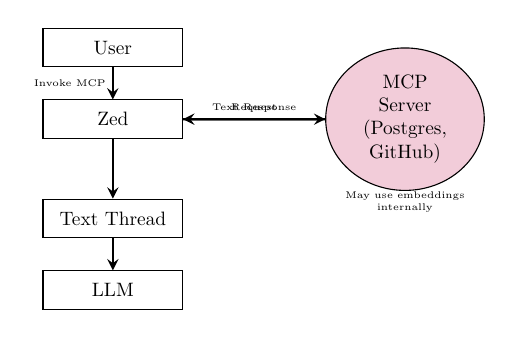
\begin{tikzpicture}[
    node distance=1.3cm,
    box/.style={rectangle, draw, text width=2.3cm, text centered, minimum height=0.7cm},
    server/.style={ellipse, draw, text width=1.8cm, text centered, minimum height=0.9cm, fill=purple!20},
    arrow/.style={->, >=stealth, thick},
    scale=0.7,
    transform shape
]
    \node[box] (user) {User};
    \node[box, below of=user] (zed) {Zed};
    \node[server, right of=zed, xshift=4cm] (mcp) {MCP Server\\(Postgres, GitHub)};
    \node[box, below of=zed, yshift=-0.5cm] (thread) {Text Thread};
    \node[box, below of=thread] (llm) {LLM};

    \draw[arrow] (user) -- node[left, font=\tiny] {Invoke MCP} (zed);
    \draw[arrow] (zed) -- node[above, font=\tiny] {Request} (mcp);
    \draw[arrow] (mcp) -- node[above, font=\tiny] {Text Response} (zed);
    \draw[arrow] (zed) -- (thread);
    \draw[arrow] (thread) -- (llm);
    
    \node[below of=mcp, yshift=-0.2cm, text width=2.2cm, text centered, font=\tiny] {May use embeddings\\internally};
\end{tikzpicture}
\caption{MCP Context Integration}
\label{fig:mcp}
\end{figure}

Key point: Zed itself doesn't manage embeddings. Any vector search happens inside the MCP server, and Zed only receives the final text result.

\section{Session Memory and Summarization}

\subsection{Thread Persistence}

Threads are stored persistently:
\begin{itemize}
    \item All messages (user, assistant, tool calls) are saved
    \item Threads can be reopened from history
    \item Previous threads can be @-mentioned to pull their content into new conversations
\end{itemize}

Zed persists threads on disk (e.g., in a local database) so they can be reopened from history. The exact storage format is an implementation detail of the open-source codebase. There is no vector database or embedding index.

\subsection{Token Pressure and Summarization}

Zed tracks token usage and shows a meter in the UI. Different models have very different context windows (e.g., 128k vs 32k), which affects how aggressive users must be about summarization. Zed recommends using purpose-based Agent threads (new thread per task) as a context-management strategy.

When approaching the model's context limit:

\begin{enumerate}
    \item Zed suggests starting a new thread
    \item The current thread can be summarized using a separate LLM call
    \item The summary becomes the starting context for the new thread
    \item From that point, the summary text is what persists as "memory"
\end{enumerate}

\begin{figure}[htbp]
\centering
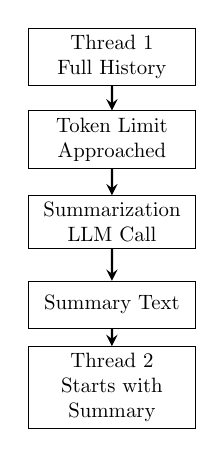
\begin{tikzpicture}[
    node distance=1.4cm,
    box/.style={rectangle, draw, text width=2.6cm, text centered, minimum height=0.8cm},
    arrow/.style={->, >=stealth, thick},
    scale=0.75,
    transform shape
]
    \node[box] (thread1) {Thread 1\\Full History};
    \node[box, below of=thread1] (token) {Token Limit\\Approached};
    \node[box, below of=token] (summarize) {Summarization\\LLM Call};
    \node[box, below of=summarize] (summary) {Summary Text};
    \node[box, below of=summary] (thread2) {Thread 2\\Starts with Summary};

    \draw[arrow] (thread1) -- (token);
    \draw[arrow] (token) -- (summarize);
    \draw[arrow] (summarize) -- (summary);
    \draw[arrow] (summary) -- (thread2);
\end{tikzpicture}
\caption{Thread Summarization Flow}
\label{fig:summarization}
\end{figure}

This is rolling textual summarization, not vector-based retrieval. Long-term memory is implemented as text summaries that users can see and edit.

\section{Complete Context Flow}

Putting it all together, here's how context flows from user input to the LLM:

\begin{figure}[htbp]
\centering
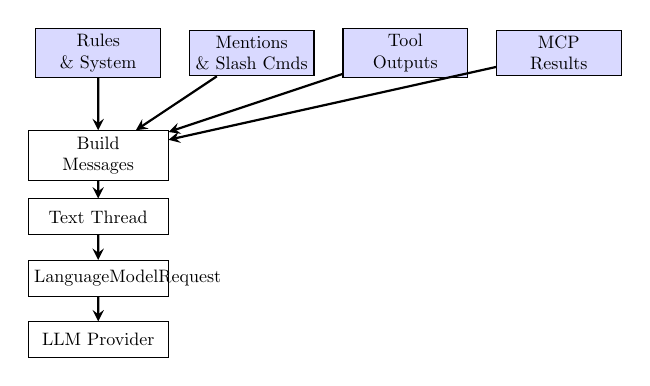
\begin{tikzpicture}[
    node distance=1.2cm,
    box/.style={rectangle, draw, text width=2.5cm, text centered, minimum height=0.7cm},
    source/.style={rectangle, draw, text width=2.2cm, text centered, minimum height=0.6cm, fill=blue!15},
    arrow/.style={->, >=stealth, thick},
    scale=0.65,
    transform shape
]
    \node[source] (rules) {Rules\\\& System};
    \node[source, right of=rules, xshift=1.8cm] (mentions) {Mentions\\\& Slash Cmds};
    \node[source, right of=mentions, xshift=1.8cm] (tools) {Tool\\Outputs};
    \node[source, right of=tools, xshift=1.8cm] (mcp) {MCP\\Results};
    \node[box, below of=rules, yshift=-0.8cm] (build) {Build\\Messages};
    \node[box, below of=build] (thread) {Text Thread};
    \node[box, below of=thread] (request) {LanguageModelRequest};
    \node[box, below of=request] (llm) {LLM Provider};

    \draw[arrow] (rules) -- (build);
    \draw[arrow] (mentions) -- (build);
    \draw[arrow] (tools) -- (build);
    \draw[arrow] (mcp) -- (build);
    \draw[arrow] (build) -- (thread);
    \draw[arrow] (thread) -- (request);
    \draw[arrow] (request) -- (llm);
\end{tikzpicture}
\caption{Complete Context Assembly Pipeline}
\label{fig:complete}
\end{figure}

The final request contains:
\begin{enumerate}
    \item \textbf{System messages}: Built from rules, project context, and system metadata
    \item \textbf{User messages}: Current input plus any retained history
    \item \textbf{Assistant messages}: Previous model responses (if kept)
    \item \textbf{Context blocks}: Resolved mentions, slash commands, tool outputs, MCP results
    \item \textbf{Tool schemas}: Available tools and their definitions
\end{enumerate}

Everything is visible in the Agent Panel—there are no hidden context layers.

\section{Online vs Offline: Context Consistency}

The context building process is identical regardless of whether the model is online or offline:

\begin{itemize}
    \item \textbf{Online (hosted)}: Same text-thread pipeline, full tool support
    \item \textbf{Offline (Ollama/LM Studio)}: Same text-thread pipeline, tools work if model supports them
    \item \textbf{Offline (no tools)}: Same text-thread pipeline, but only explicit context (no automatic tool calls)
    \item \textbf{External agents (ACP)}: Context forwarded via ACP, may have different capabilities
\end{itemize}

The difference is in transport and tool capabilities, not in how context is built or stored.

\section{Security and Privacy of Context}

The text-first approach makes it easier to audit what data leaves your machine:

\begin{itemize}
    \item \textbf{What's sent}: Everything in the thread, attached files, rules, and tool outputs included in the request
    \item \textbf{Hosted models}: Data sent to OpenAI, Anthropic, etc. (their privacy policies apply)
    \item \textbf{Self-hosted}: Data stays local (Ollama, LM Studio)
    \item \textbf{MCP servers}: Run as separate processes and may log/store what they receive—they're not automatically trusted
    \item \textbf{External agents}: Forward context via ACP; their privacy policies apply
\end{itemize}

Since all context is visible in the thread, users can review exactly what will be sent before making a request.

\section{Text-First vs RAG-First: Tradeoffs}

Zed explicitly does not include built-in vector stores or automatic RAG. This design choice has clear tradeoffs:

\subsection{Advantages}

\begin{itemize}
    \item \textbf{Debuggability}: See exactly what context the model received
    \item \textbf{Control}: Decide what context to include, when, and how
    \item \textbf{Predictability}: No hidden behavior that's hard to reason about
    \item \textbf{Editability}: Rewrite history before resending
    \item \textbf{Composability}: Context sources (rules, files, tools, MCP) are clearly separated
    \item \textbf{Token transparency}: See token usage and optimize accordingly
\end{itemize}

\subsection{Costs}

\begin{itemize}
    \item \textbf{Manual curation}: Users (or tools) must curate context—easier to miss important files in huge monorepos
    \item \textbf{Token usage}: Can explode if people @directory everything without filtering
    \item \textbf{No automatic semantic search}: Must bring MCP/external RAG for semantic retrieval across millions of lines
\end{itemize}

\subsection{Hybrid Approaches}

If you need vector search or semantic retrieval:
\begin{itemize}
    \item Use an MCP server that implements it (returns compact textual digest)
    \item Build a custom Agent Server that does embeddings internally
    \item Use BMAD-style documentation methods that convert semantic structure into textual knowledge
\end{itemize}

This keeps RAG opt-in and transparent, rather than hidden in the core system.


\section{Conclusion}

Zed's context management architecture demonstrates that sophisticated AI assistance doesn't require hidden embedding systems or opaque vector stores. By making context explicit, editable, and visible, Zed gives users the control and transparency needed to effectively work with language models.

The text-first approach means:
\begin{itemize}
    \item Context is built from explicit text inclusion (manual or tool-driven)
    \item Everything is visible in the Agent Panel or Text Threads
    \item Memory is stored as editable text threads
    \item Long-term context uses summarization, not vectors
    \item External embeddings (via MCP) are opt-in and transparent
    \item Automatic context gathering is observable, not hidden
\end{itemize}

This architecture provides a solid foundation for building reliable, debuggable AI-powered development tools while maintaining user control and system transparency. The tradeoff is that users must be more deliberate about context curation, but gain complete visibility and control over what the model sees.

\end{document}

